\begin{appendices}
	\chapter{Приложение А}
	Примеры работы реализации алгоритма шифрования машиной Enigma.
	
\begin{table}[H]
	\centering
	\begin{tabular}{p{1\linewidth}}
		\centering
		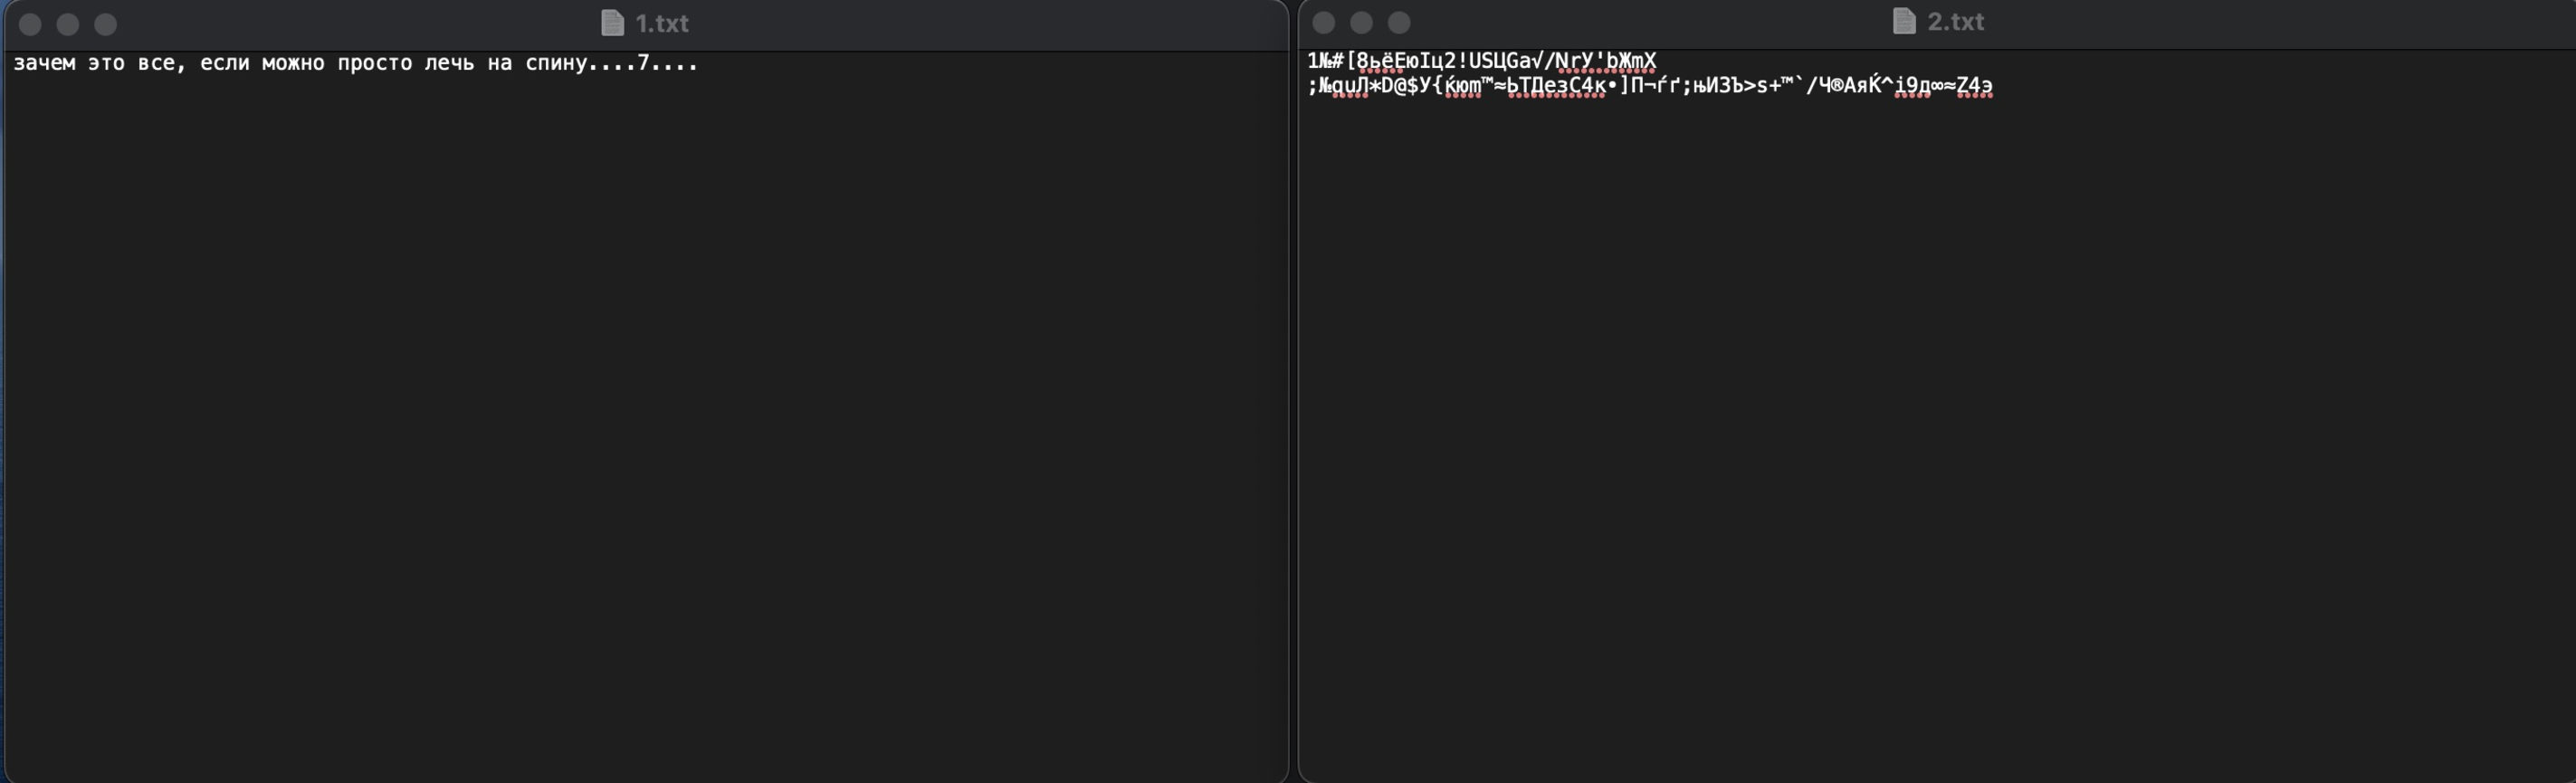
\includegraphics[width=0.9\linewidth]{inc/pdfs/1.pdf}
		\captionof{figure}{txt файл на русском}
		\label{img:enigma}
	\end{tabular}
\end{table}

\begin{table}[H]
	\centering
	\begin{tabular}{p{1\linewidth}}
		\centering
		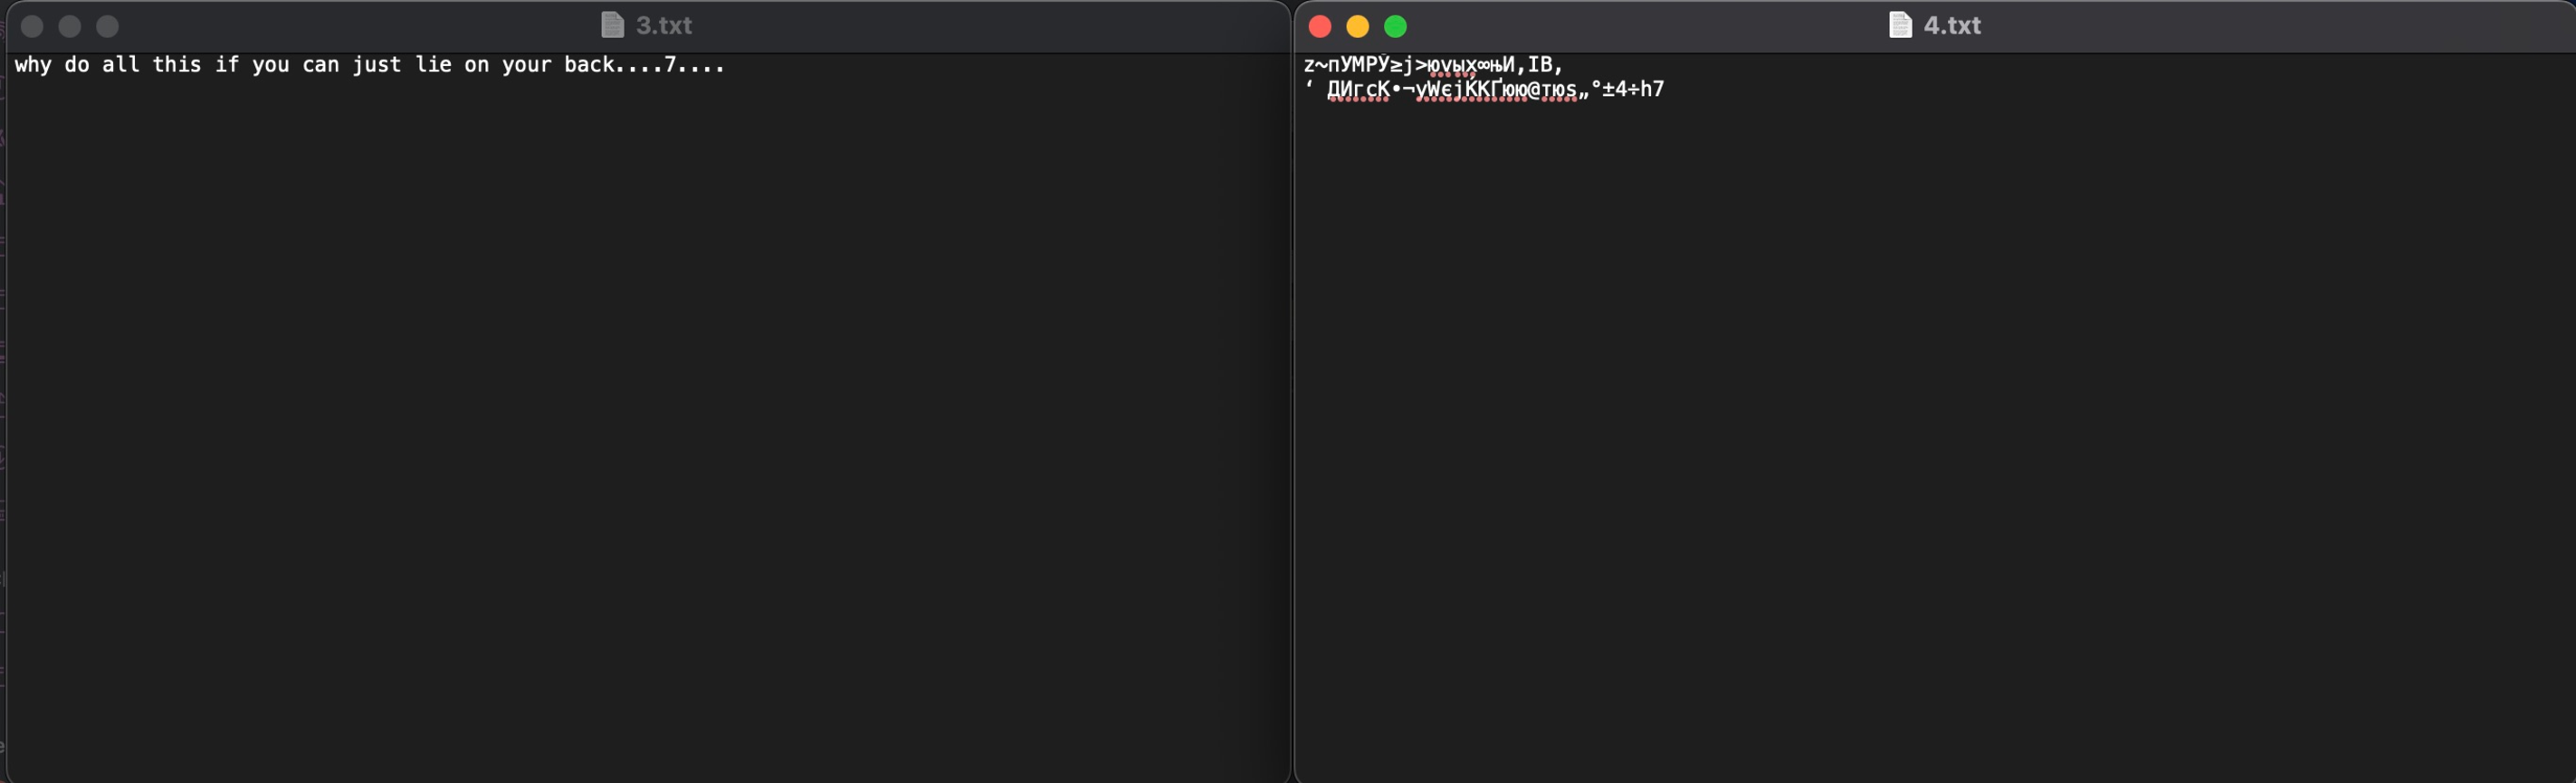
\includegraphics[width=0.9\linewidth]{inc/pdfs/2.pdf}
		\captionof{figure}{txt файл на английском}
		\label{img:enigma}
	\end{tabular}
\end{table}

\begin{table}[H]
	\centering
	\begin{tabular}{p{1\linewidth}}
		\centering
		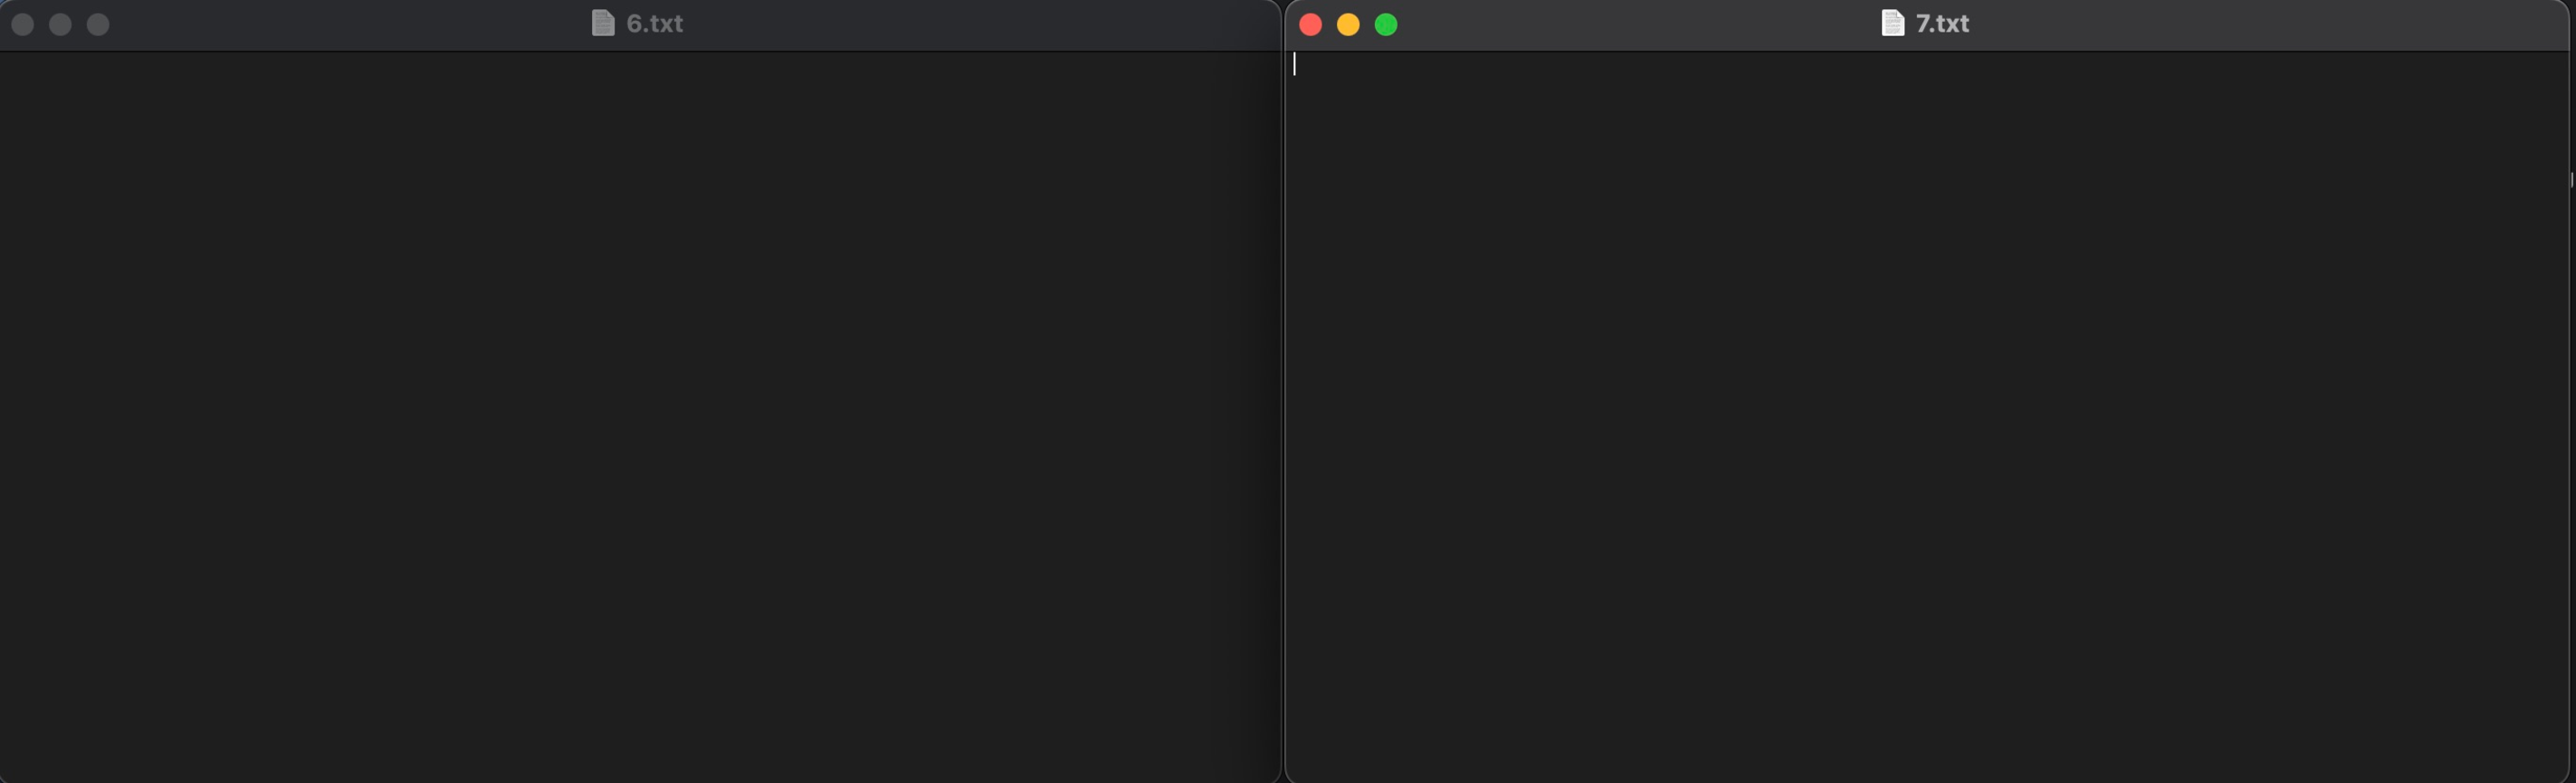
\includegraphics[width=0.9\linewidth]{inc/pdfs/3.pdf}
		\captionof{figure}{Пустой файл}
		\label{img:enigma}
	\end{tabular}
\end{table}

\begin{table}[H]
	\centering
	\begin{tabular}{p{1\linewidth}}
		\centering
		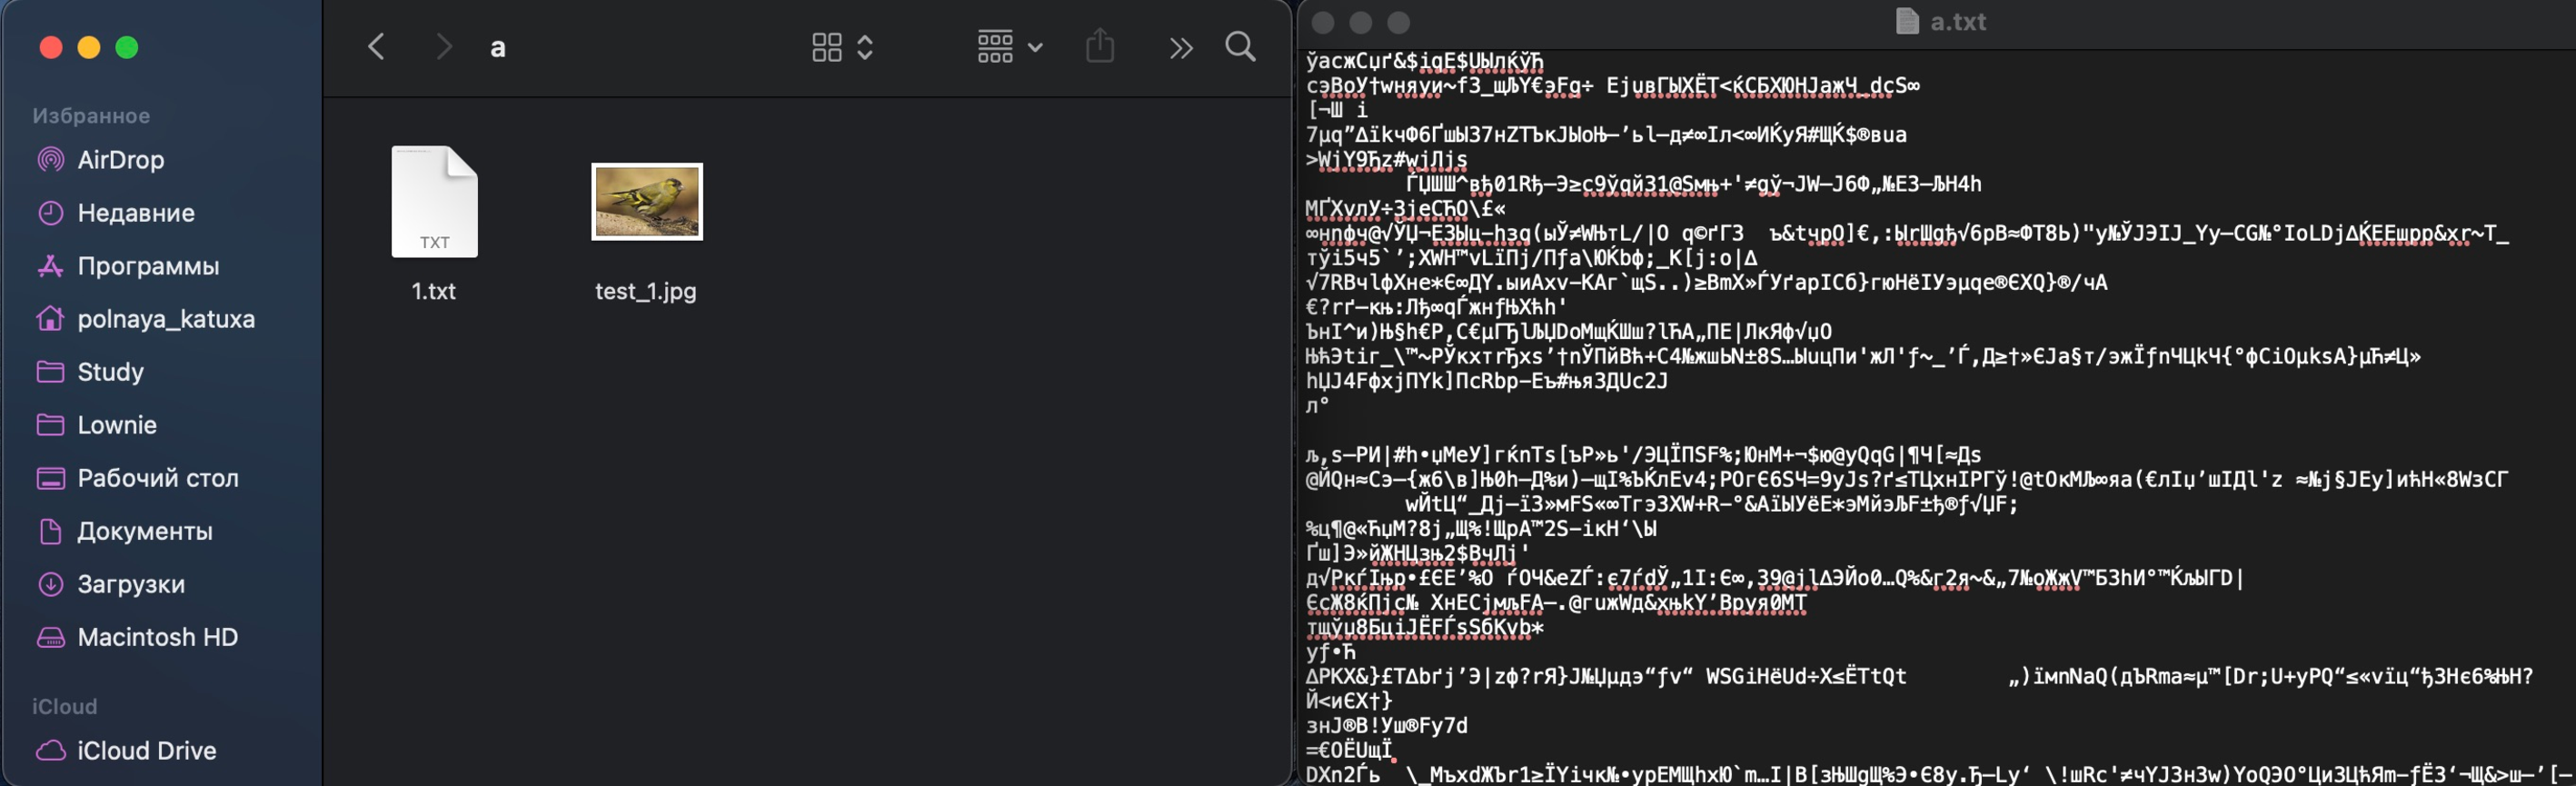
\includegraphics[width=0.9\linewidth]{inc/pdfs/4.pdf}
		\captionof{figure}{zip архив с двумя файлами}
		\label{img:enigma}
	\end{tabular}
\end{table}

\begin{table}[H]
	\centering
	\begin{tabular}{p{1\linewidth}}
		\centering
		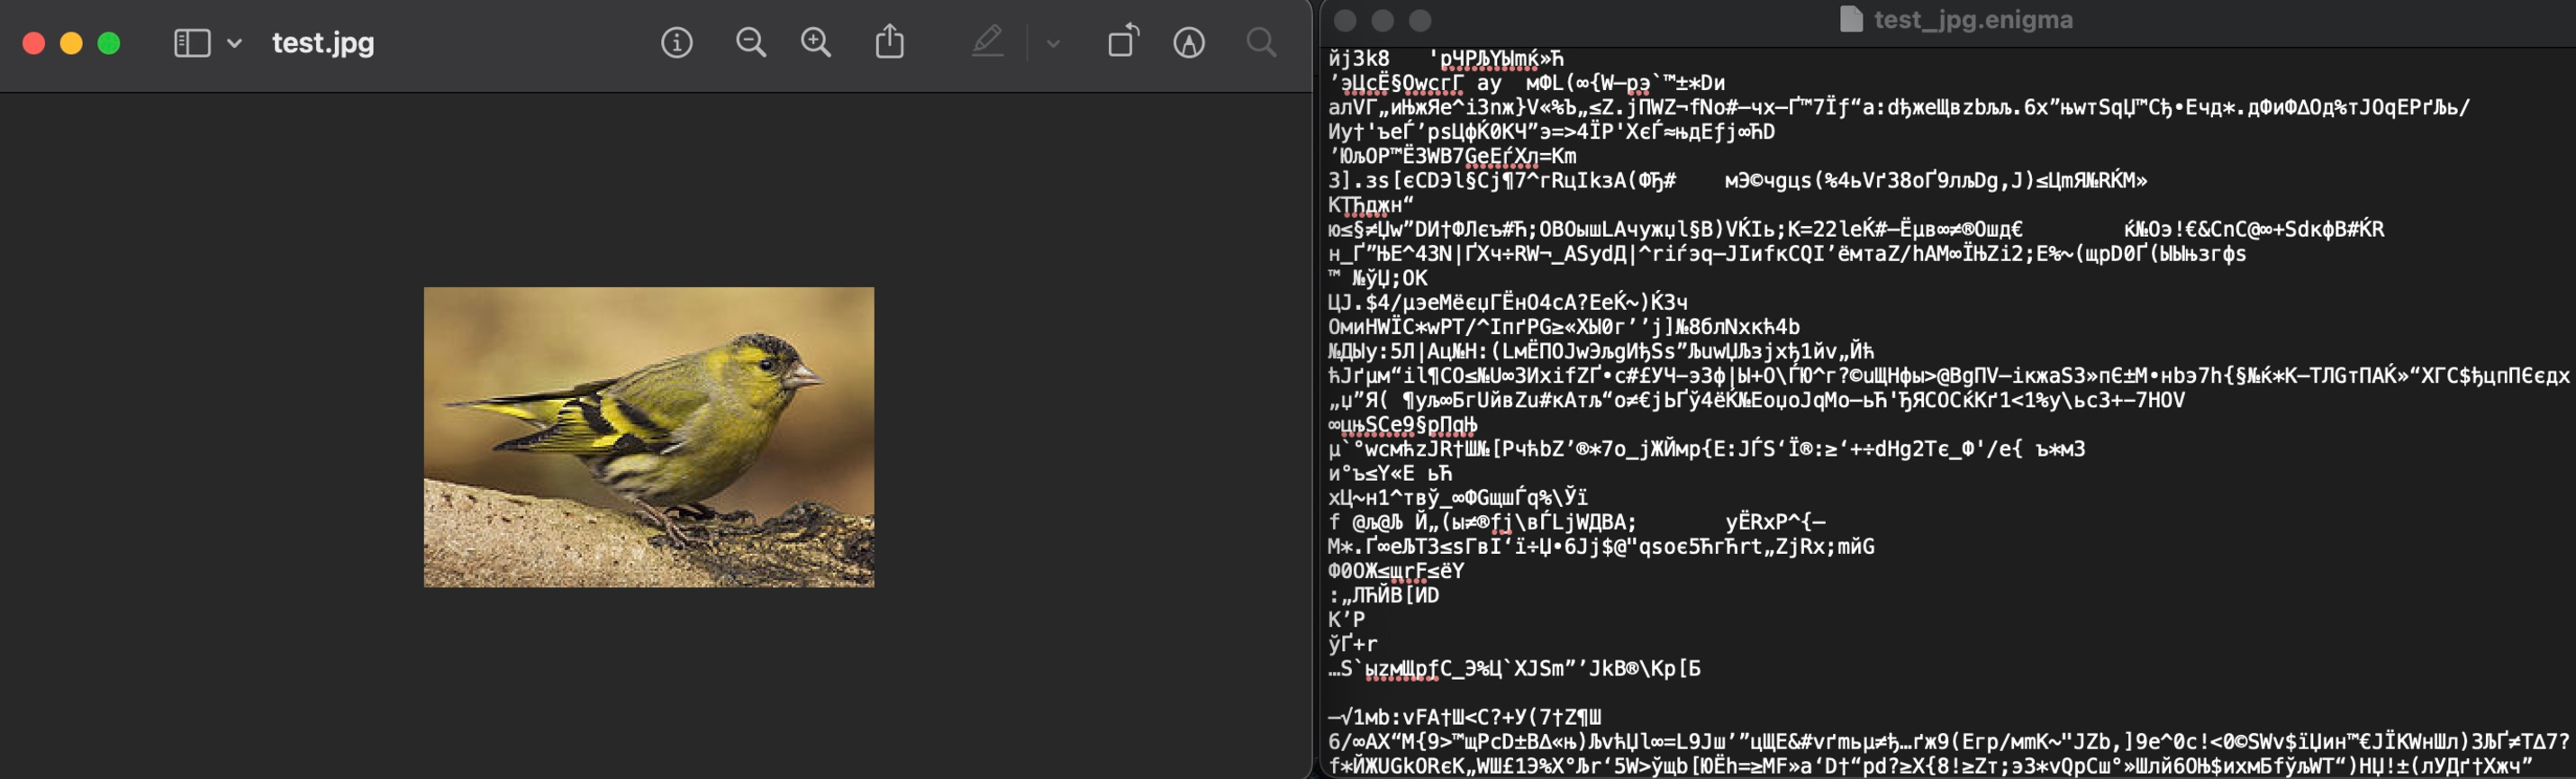
\includegraphics[width=0.9\linewidth]{inc/pdfs/5.pdf}
		\captionof{figure}{jpg изображение}
		\label{img:enigma}
	\end{tabular}
\end{table}

\begin{table}[H]
	\centering
	\begin{tabular}{p{1\linewidth}}
		\centering
		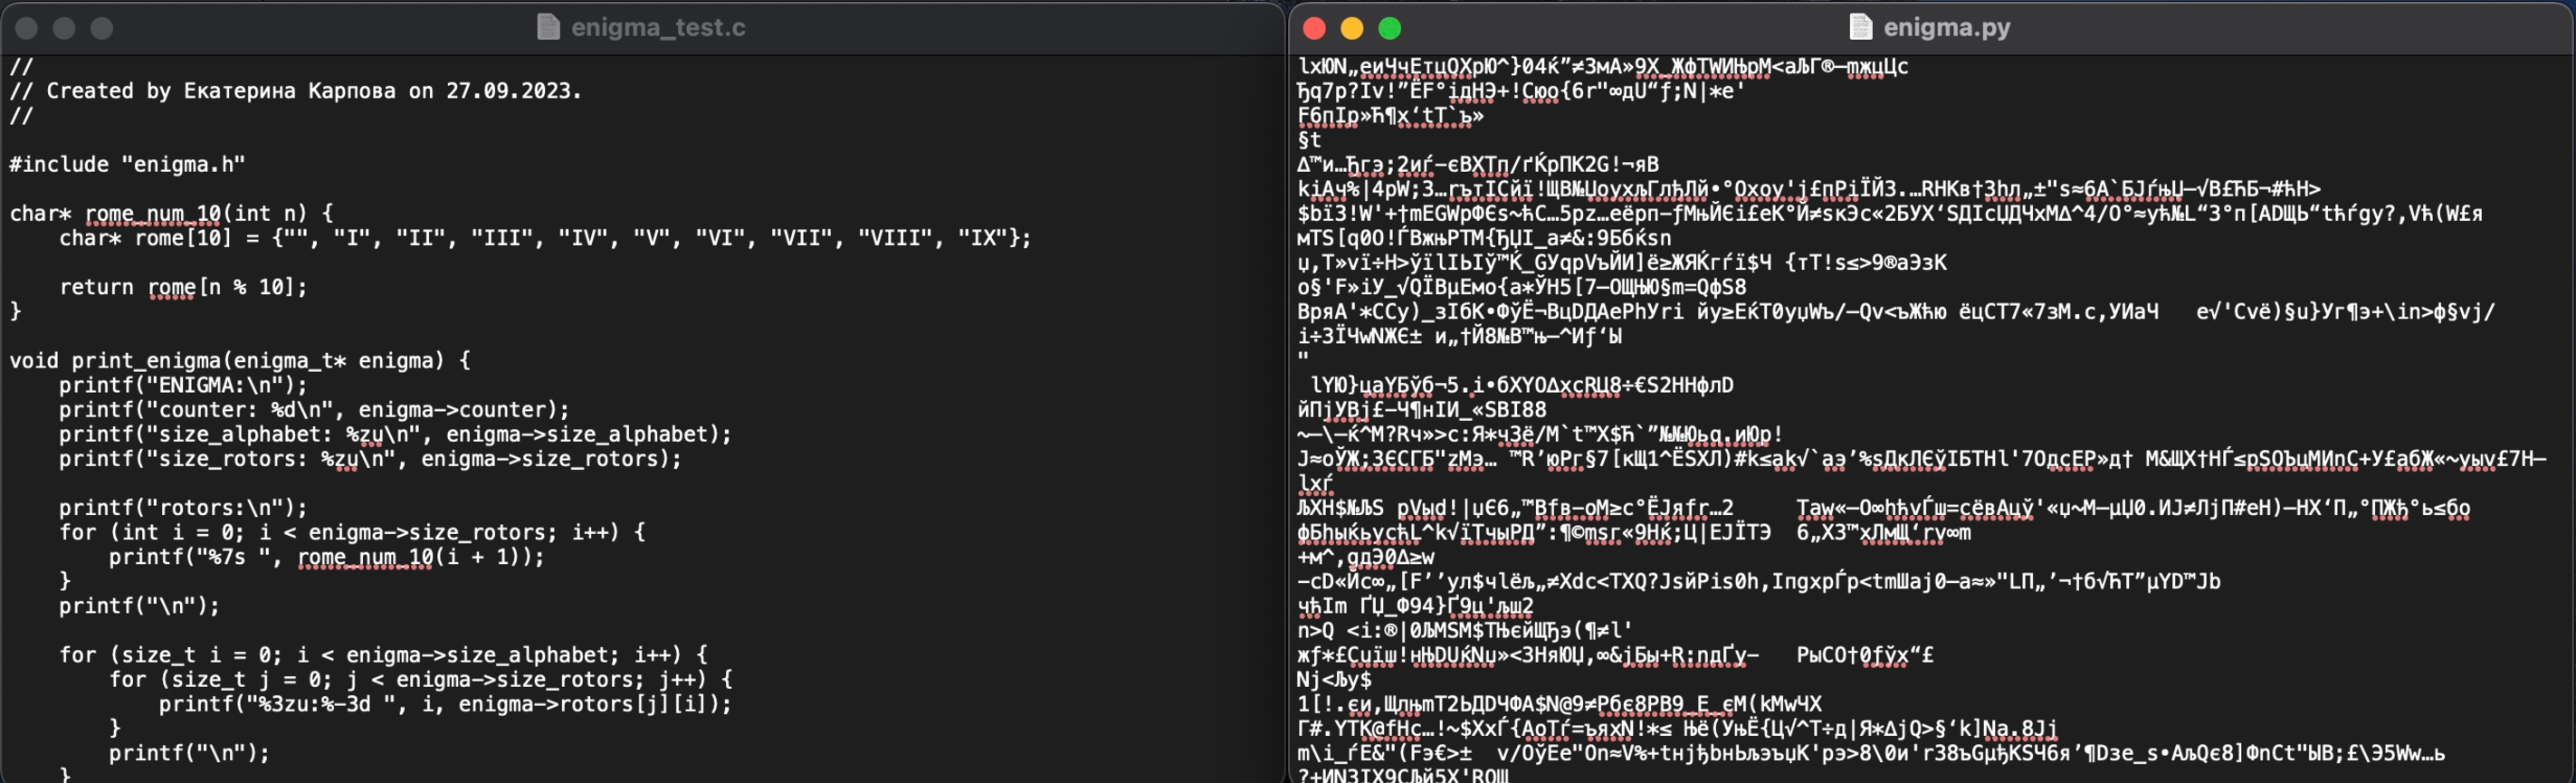
\includegraphics[width=0.9\linewidth]{inc/pdfs/6.pdf}
		\captionof{figure}{Файл исходного кода на языке C}
		\label{img:enigma}
	\end{tabular}
\end{table}

\begin{table}[H]
	\centering
	\begin{tabular}{p{1\linewidth}}
		\centering
		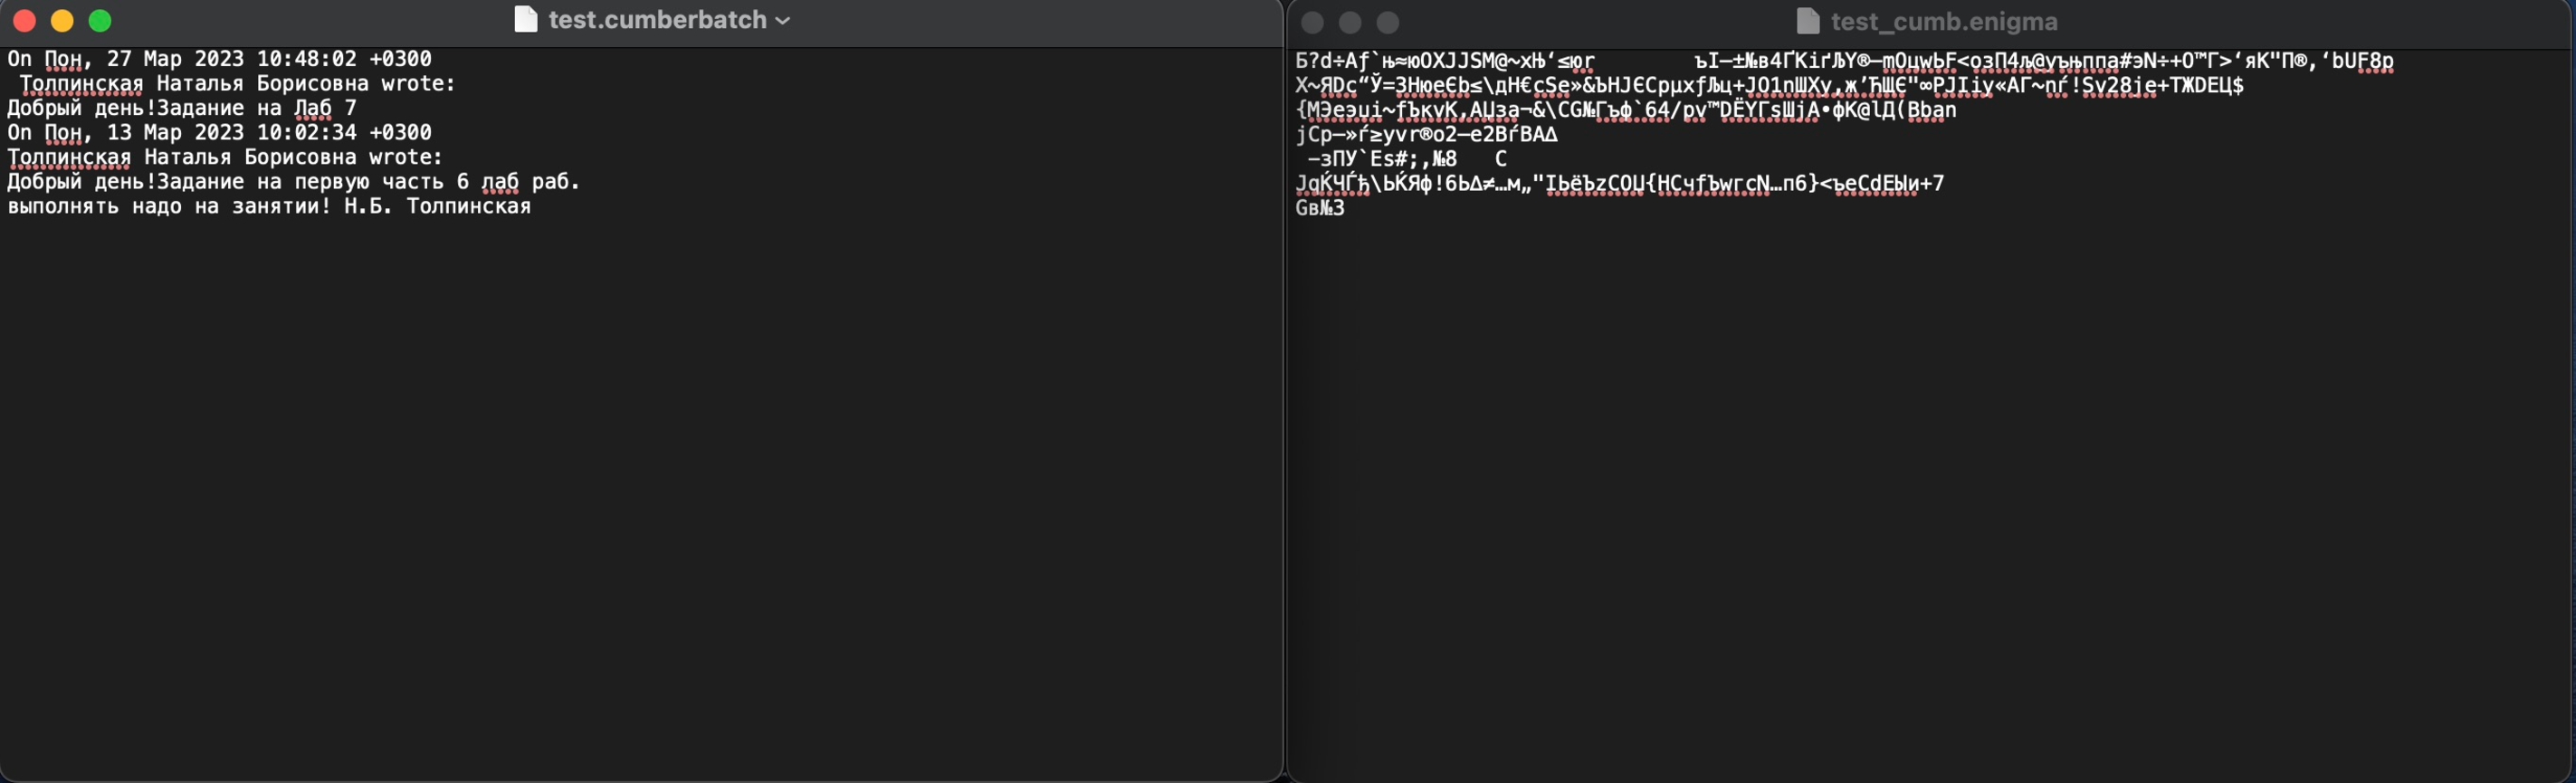
\includegraphics[width=0.9\linewidth]{inc/pdfs/7.pdf}
		\captionof{figure}{Файл с выдуманным расширением}
		\label{img:enigma}
	\end{tabular}
\end{table}

\begin{table}[H]
	\centering
	\begin{tabular}{p{1\linewidth}}
		\centering
		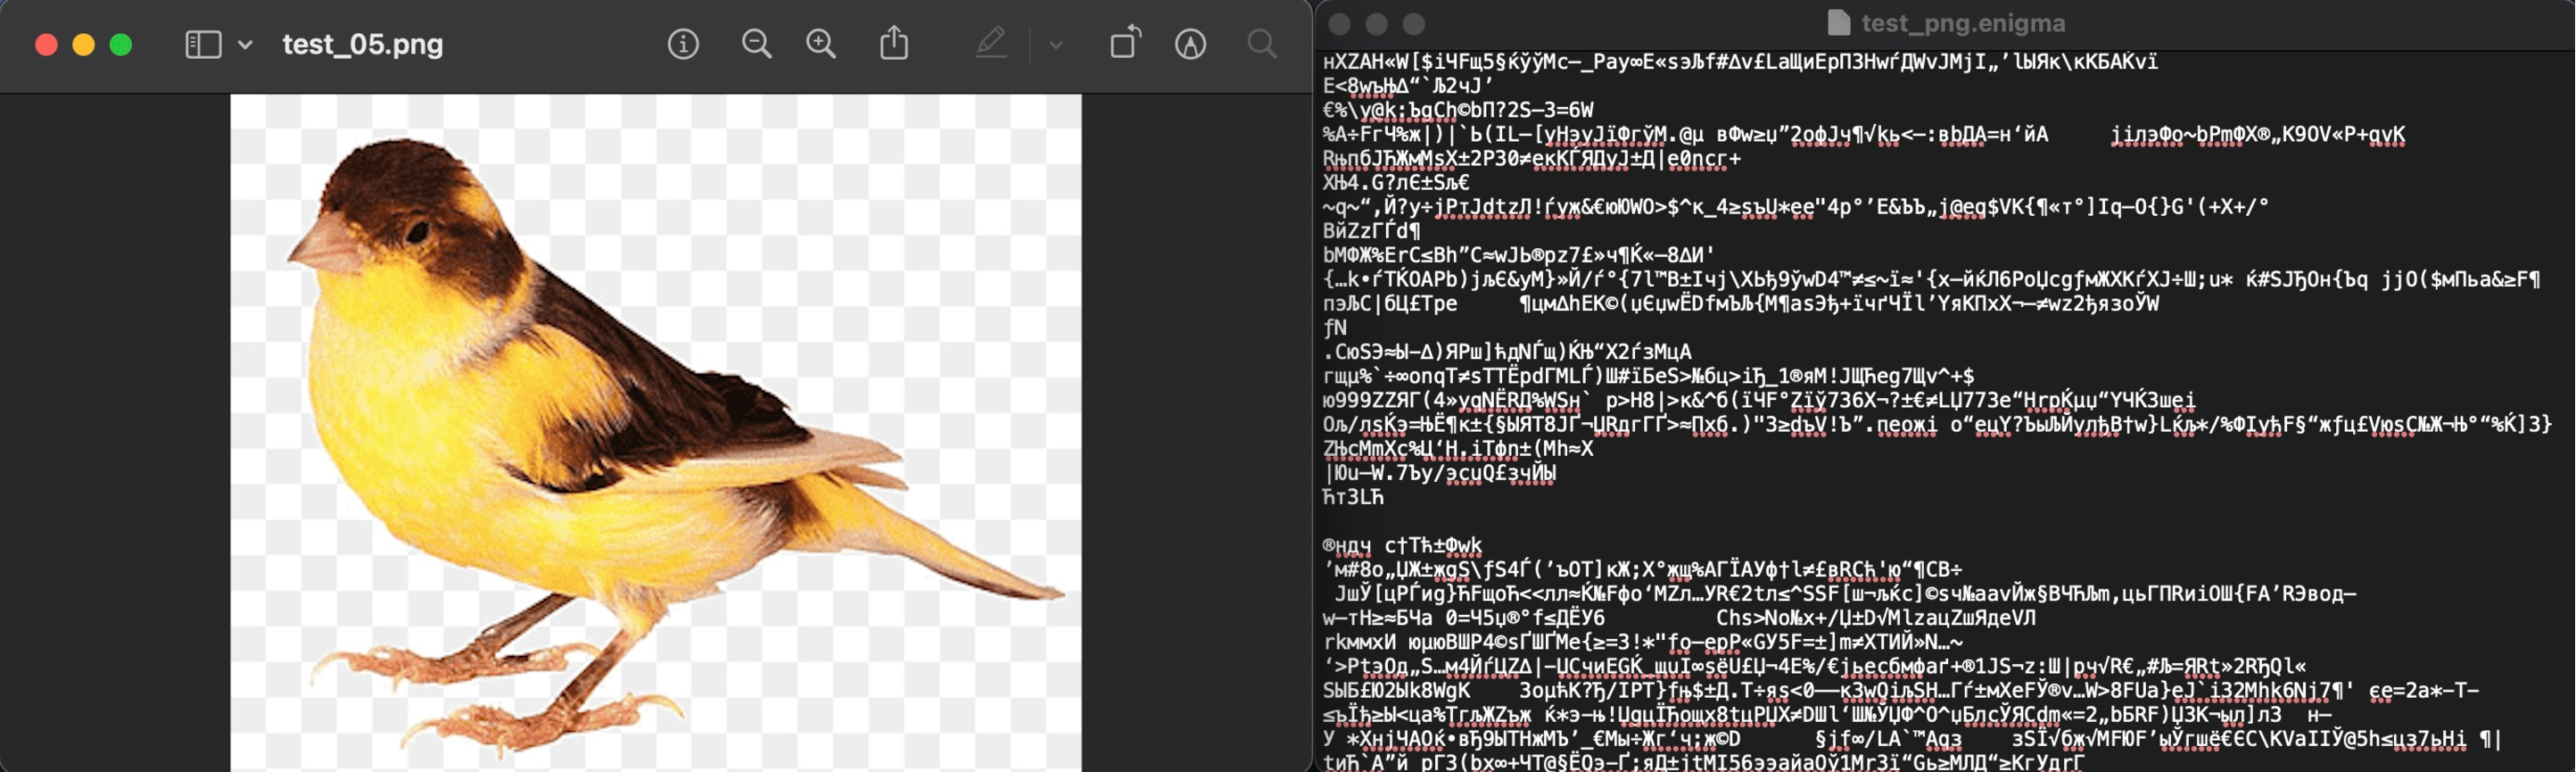
\includegraphics[width=0.9\linewidth]{inc/pdfs/8.pdf}
		\captionof{figure}{png изображение}
		\label{img:enigma}
	\end{tabular}
\end{table}
	
\end{appendices}